
\documentclass{beamer}
\usetheme{umbc1}

%%% Packages
% First four - AMS (american mathematical society). General math goodness. I use the align* enviorment in particular
% multirow, multicol allow for certain kinds of tables
% enumerate lets you determine the style of the counter for the enumerate enviorment
% graphicx lets you include pictures
% listings lets you stick in blocks of code
% placeins defines "\FloatBarrier", which stops tables from moving around
\usepackage{amsmath, amscd, amssymb, amsthm, multirow, multicol, enumerate, graphicx, listings, placeins} 
\newcommand{\Z}{\mathbb{Z}}
\newcommand{\R}{\mathbb{R}}
\newcommand{\Q}{\mathbb{Q}}
\newcommand{\C}{\mathbb{C}}
\newcommand{\N}{\mathbb{N}}
\newcommand{\V}{\mathbb{V}}
\newcommand{\U}{\mathcal{U}}
\newcommand{\del}{\partial}
\newcommand{\real}{\textrm{Re }}
\newcommand{\imag}{\textrm{Im }}
\newcommand{\pd}[2]{\frac{\partial #1}{\partial #2}}
\newcommand{\deriv}[2]{\frac{d #1}{d #2}}
\newcommand{\sumk}{\sum_{k=1}^\infty}
\newcommand{\sumj}{\sum_{j=1}^\infty}
\newcommand{\sumn}{\sum_{n=0}^\infty}
\newcommand{\summ}[2]{\sum_{k=#1}^{#2}}
\newcommand{\sig}[1]{\sum_{#1 =1}^\infty}
\newcommand{\un}[1]{\bigcup_{#1 =1}^\infty}
\newcommand{\inter}[1]{\bigcap_{#1 =1}^\infty}
\newcommand{\ip}[2]{\langle #1, #2 \rangle}
\newcommand{\ipxu}{\langle x,u_j \rangle}
\newcommand{\uj}{\{u_j\}_{j=1}^\infty}
\newcommand{\B}{\mathcal{B}}

\newcommand{\E}{\mathrm{E}}
\newcommand{\var}{\mathrm{Var}}
\newcommand{\cov}{\mathrm{Cov}}
\newcommand{\ST}{mbox{ s.t. }}

\newcommand{\st}{ \; \big | \:}

\newcommand{\deuc}{d_{\mathrm euc}}
\newcommand{\dtaxi}{d_{\mathrm taxi}}
\newcommand{\ddisc}{d_{\mathrm disc}}

\newcommand{\hwhead}[1]{#1 \hfill Aaron Maurer \vspace{2mm} \hrule \vspace{2mm}}
\newcommand{\diag}[1]{\mathrm{diag}\{#1\}}
\DeclareMathOperator*{\argmin}{arg\min}

\title{Using Probabilistic Knockoffs of Binary Variables to Control the False Discovery Rate}
\author{Aaron Maurer}
\date{July 29th, 2015}

\begin{document}
%%%%%%%%%%%%%%%%%%%%%%%%%%%%%%%%%%%%%%%%%%%%%%%%%%%%%%%%%%%%%%%%%%%%%%%%%%%%%%%%%%%%%%%%%%%%%%%%%%%%%%%%%%%%%%%%%%%%%%%%%%%%%%%%%%%%%
\begin{frame}[plain]
    \titlepage
\end{frame}

\begin{frame}{Overview}
    \begin{enumerate} 
        \item Original Knockoffs: What They Do and Where They Fail
        \item Making Knockoffs Work With GLMs
        \item Random Binary Knockoffs: The Theory
        \item Random Binary Knockoffs: Performance
        \item Where to next?
    \end{enumerate}
\end{frame}

\begin{frame}{Variable Selection in Linear Regression}
    Assume
     \[\mathbf{y} = X\beta + \mathbf{z}\]
    where $\mathbf{y}\in\R^n$, $X \in \R^{n\times p}$, $\beta\in\R^p$, and $\mathbf z$ is Gaussian noise. Also, assume sparsity:
    \[\beta_i = 0 \quad \forall i\not\in S\]
    How do we pick estimate $\hat S$?
\end{frame}

\begin{frame}{False Discover Rate}
    A common goal for a method that generates $\hat S$ is to control the false discovery rate
    \[ \textrm{FDR} = \E\left[\frac{\vert{\{j: \beta_j=0 \; \& \; j\in\hat S\}}\vert}{\max\{\vert{\hat S}\vert,1\}} \right] \]
    In other words, control portion of elements in $\hat S$ which aren't in $S$. \par
    \vspace{1cm}
    FDR is controlled at level $q$ if $q<$FDR irrespective of true $\beta$.
    
\end{frame}

\begin{frame}{Knockoffs}
    Knockoff variables can be used to control FDR in linear regression. 
    \begin{itemize}
        \item The idea is to create a forgery of each variable; if the forgeries seem about as good predictors as the originals, the originals are lousy predictors.
        \item For each variable $X_i$, create a knockoff feature $\tilde X_i$. Such that. 
            \[ \tilde X^T \tilde X = X^T X \quad \& \quad X^T \tilde X = X^T X - \diag{\mathbf s} \]
            Where $\diag{X^T X} - s$ is small but $\diag{X^T X} - s\succeq0$
        \item $\tilde X_i$ and $X_i$ will have same correlation with other variables, but only low correlation with each other.
        \item Given $\mathbf s$, $\tilde X$ can be generated via a rotation of $X$.
    \end{itemize}
\end{frame}

\begin{frame}{Knockoff Filter}
    These knockoffs can be used in the knockoff filter method. 
    \begin{itemize}
        \item Fit full path of LASSO regression on $[\,X\,\tilde X\,]$.
    \[ \beta(\lambda) = \argmin_\mathbf b \left\{\frac{1}{2}\|\mathbf y - X_L\mathbf b\|^2_2 + \lambda\|b\|_1 \right\}\]
        \item $Z_i$, $\tilde Z_i$ largest $\lambda$ such that $X_i$, $\tilde X_i$ have nonzero coefficient.
        \item $W_i= Z_i$ if $Z_i>\tilde Z_i$, otherwise $W_i = -\tilde Z_i$.
        \item Since $[\, X \, \tilde X\,]^T[\, X \, \tilde X\,]$ \& $[\, X \, \tilde X\,]^T\mathbf y$ sufficient statistics for $\beta(\lambda)$, $W_i$ symmetrically distributed around $0$ when $X_i$ null predictor.
        \item Thus, FDR controlled when $\hat S = \{i:W_i>T\}$ for 
            \[ T = \min\left\{ t>0 \;: \; \frac{\vert\{j:W_j\leq -t\}\vert}{\max\{\vert\{j:W_j\geq t\}\vert,1\}}\leq q \right\} \]
    \end{itemize}
\end{frame}

\begin{frame}{Where Knockoff Filter Fails}
    Knockoff filter don't work for other GLMs. \\
    \begin{center}
        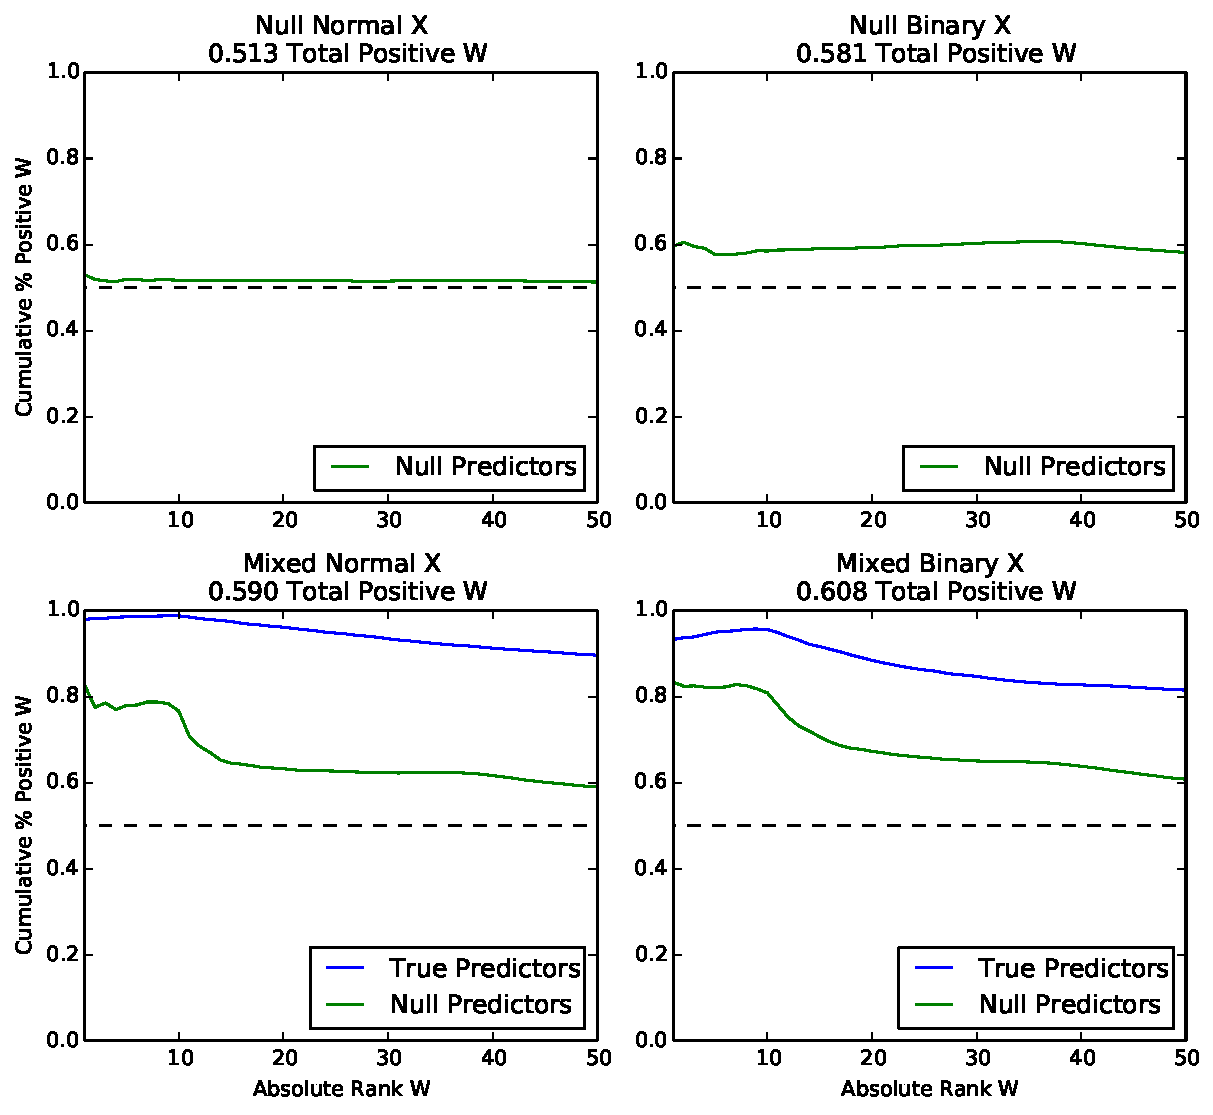
\includegraphics[width=8cm]{images/entryrate_original_logit}
    \end{center}
\end{frame}

\begin{frame}{Can Knockoffs Be Fixed for GLMs?}
    \begin{itemize}
        \item Other GLMs don't have the same sufficient statistics as linear regression.
        \item Original Knockoffs don't remotely have same distribution as $X$, so ``look'' different than real variables.
        \item Knockoffs will likely work better if they have the same marginal distribution as originals. 
        \item For $X_i$ with arbitrary distribution, unclear how this might be accomplished.
    \end{itemize}
\end{frame}

\begin{frame}{Random Binary Knockoffs}
    \begin{itemize}
        \item A useful 
    \end{itemize}
\end{frame}



\end{document}
